\documentclass[10pt,a4paper]{article}

\usepackage[english,italian]{babel}
\usepackage[utf8]{inputenc}
\usepackage[T1]{fontenc}

\usepackage{comment}

%------Liste------
\usepackage{enumitem} %lists

%------Figure------
\usepackage{graphicx} %img/media

%------Math------
\usepackage{mathtools} %math package
\usepackage{amssymb} %pacchetto per i simboli di matematica
\usepackage{amsmath} %pacchetto di matematica
\usepackage{amsthm} %pacchetto di matematica\raggedbottom

%------CodeEnviroment----
\usepackage{listings} %coding environment 
\usepackage{xcolor} %define colors

%-------Margini------
\usepackage{geometry}
%\geometry{a4paper,top=1.5cm,bottom=2.5cm,left=1.5cm,right=1.5cm,heightrounded}
\raggedbottom

%------Tabelle------
\usepackage{booktabs} %toprule e midrule usati al posto di hline
\usepackage{float} %oggetti mobili(tabelle, figure etc)
\usepackage{longtable,tabu} %tabelle lunghe su più pagine
\usepackage{tabularx} %tabelle larghe

%------Indice----
\usepackage{hyperref} %linkare l indice
\hypersetup{hidelinks} %nascondere i link dell'indice


\title{Progetto di Programmazione a Oggetti}
\author{Sara Righetto, matricola 1174009}
\date{Anno accademico 2018/2019}

\begin{document}
    \maketitle
    \begin{abstract}
        QPlay è un applicazione che consente, tramite l'uso di un contenitore, la gestione e visualizzazione di file audio-visivi di vario tipo. L'utente può inserire, modificare, eliminare file, eseguire ricerche in base a diversi campi dati e caricare/salvare su disco la propria lista di file personale.
    \end{abstract}

    \section*{Gerarchia dei tipi}
        La gerarchia vuole modellare degli oggetti che comprendono alcuni file audio-visivi ed è così composta: una classe base astratta denominata \texttt{AudioVisual} e tre classi derivate concrete \texttt{TvSerie}, \texttt{Movie}, \texttt{Documentary} che implementano i metodi puri della classe base. 

\begin{center}
    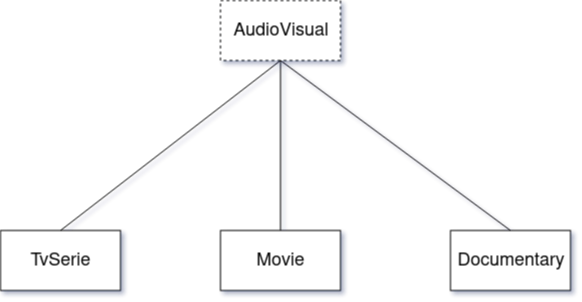
\includegraphics[width=0.6\textwidth]{gerarchia}
\end{center}

\paragraph{AudioVisual}
La classe base della gerarchia fornisce le informazioni di base comuni a tutti i file di tipo audio-visivo, ossia il \textit{titolo} del file, il percorso dell'\textit{immagine} di copertina, la \textit{descrizione} della trama, l'\textit{anno} di uscita, la \textit{durata} in minuti, il nome del \textit{regista}, l'appartenenza ai \textit{preferiti} dell'utente, se l'audio è \textit{compresso} o meno, la \textit{risoluzione} dell'immagine, i \textit{frame per secondo}.

\paragraph{TvSerie}
TvSerie è una classe derivata concreta che rappresenta i file riguardanti le serie tv, infatti aggiunge i campi dati riguardanti il numero di \textit{episodi} della serie, il numero di \textit{stagioni}, se la serie è \textit{terminata}, il \textit{rating}, il \textit{genere}, il \textit{cast} formato dai personaggi.

\paragraph{Documentary}
Documentary è una classe derivata concreta che rappresenta i file di tipo documentario, in cui si ha un \textit{topic} che spazia dall'argomento scientifico, a quello storico o biografico e un campo dati riservato al \textit{narratore}.

\paragraph{Movie}
Movie è anch'essa una classe derivata concreta che vuole rappresentare i file di tipo film; aggiunge i campi dati riguardanti il \textit{cast}, il \textit{rating} ed il \textit{genere}. \newline

La gerarchia attuale è stata pensata per essere estensibile in futuro, sia in orizzontale, per esempio implementando una classe riguardante i video di YouTube, che in verticale, per esempio derivando da \texttt{TvSerie} una classe che rappresenti le telenovelas. \newline
Inoltre non fa uso di dati o classi riguardanti il framework QT, per cui è indipendente da esso.

\paragraph{DeepPtr}
Il progetto fa uso anche di un template di classe \texttt{DeepPtr<T>} di puntatori polimorfi al tipo T che implementano la gestione automatica della memoria cosidetta profonda. È quindi necessario che ogni classe concreta della gerarchia implementi il metodo relativo alla clonazione e anche la distruzione polimorfa.

\paragraph{Polimorfismo}
All'interno della gerarchia, nella classe base, sono stati dichiarati 5 metodi virtuali puri che vengono poi implementati nelle classi derivate concrete. 
\begin{enumerate}
    \item \texttt{virtual AudioVisual* clone() const =0;} utilizzato dallo \textit{SmartPointer} per la copia profonda dell'oggetto.
    \item \texttt{virtual unsigned int getTotalRunningTime() const =0;} che si occupa di calcolare la durata totale di ogni oggetto.
    \item \texttt{virtual std::string getType() const =0;} restituisce sottoforma di stringa il tipo dell'oggetto.
    \item \texttt{virtual bool isHighQuality() const =0;} che determina se un oggetto è di qualità o meno in base alla risoluzione dell'immagine, della compressione dell'audio e dei frame per secondo.
    \item \texttt{virtual bool matureContent() const =0;} si occupa di determinare se l'oggetto è visionabile solo da adulti.
\end{enumerate}
Inoltre, sebbene non siano metodi puri, sono stati dichiarati virtuali anche i metodi \texttt{virtual bool operator==(const AudioVisual\&) const;} che fa un confronto tra ogni campo dati presente nella classe e anche il distruttore.




%4k, 144p, 240, 480, 360, 720
%4k/2160p, FullHD/1080p, HD/720p, SD/480p, LD/240p


    \section*{Container<T>}
        Il contenitore templetizzato è stato sviluppato secondo la linea del contenitore \texttt{List} della libreria STL. \newline
        Il contenitore fa utilizzo delle classi annidate \texttt{Node} che rappresenta un nodo della lista, con la sua \textit{info}, il puntatore al nodo precedente \textit{prev} e al successivo \textit{next}, la classe \texttt{Iterator} e \texttt{Const\_Iterator} usate per scorrere gli elementi della lista.
        Come da specifica offre metodi per l'inserimento di nodi, quali \texttt{push\_front} e \texttt{push\_back}, la rimozione di nodi tramite \texttt{clear}, \texttt{erase}, \texttt{pop\_front} e \texttt{pop\_back}, e la ricerca di elementi grazie all'uso di \texttt{search} sia const che non. \newline
        Sebbene il contenitore venga utilizzato istanziandolo con parametro uguale a \texttt{DeepPtr<AudioVisual>}, il parametro T può assumere qualsiasi tipo, che sia primitivo o definito dall'utente.
        %Double linked list per sostenere meglio i costi per la rimozione dei nodi in posizione arbitraria.

    \section*{Persistenza delle informazioni}
        Come da specifica il progetto consente il caricamento e salvataggio delle informazioni relative al contenitore. Si è scelto di adottare l'uso dei file \textsc{xml} come formato di file per la persistenza. \newline
        Sono state implementate le funzioni \texttt{load} e \texttt{save} che fanno uso delle classi \texttt{QXmlStreamWriter} e \texttt{QXmlStreamReader} per la codifica e decodifica del file \textsc{xml}, e le classi \texttt{QFile} e \texttt{QSaveFile} per l'apertura e in generale la gestione dei file. \newline
        Entrambe le funzioni devono essere chiamate esplicitamente dall'utente e avvengono in automatico, tranne all'uscita dell'applicazione in cui tramite un popup apposito viene chiesto se si vuole salvare o meno i dati correnti.

    \section*{GUI}
        Per lo sviluppo della parte relativa alla GUI è stato adottato il design pattern \textit{Model-View}. \newline
        La parte grafica si compone di una \texttt{MainWindow} principale che viene lanciata all'avvio dell'applicazione, da \texttt{AddDialog} che si occupa di inserire nuovi oggetti nella collezione, da \texttt{AudioVisualItem} che si occupa di mostrare i dettagli principali di ciascun oggetto contenuto nella lista, da \texttt{EditWidget} che si occupa di modificare un singolo elemento della lista, da \texttt{DisplayWidget} che si occupa di visualizzare tutti i dettagli di un oggetto. \newline
        %Sia per la rimozione che per la ricerca non mi è stato necessario creare altre classi e widget all'infuori di quelli sopra descritti.
        %Da qui, nella barra in alto si può scegliere se caricare, salvare od uscire dall'applicazione.

        %insert, remove, find, edit

    \section*{Ambiente di sviluppo e direttive di compilazione}
        Il progetto è stato sviluppato su sistema operativo Manjaro Linux, utlizzando l'IDE \textit{QtCreator} con il relativo framework QT v. 5.12 e compilatore GCC v. 9.1.0. \newline
        Poichè il progetto fa ampio uso di alcune \textit{keywords} di C++11 (per esempio \texttt{auto} e \texttt{nullptr}) viene fornito il file \texttt{.pro} da compilare tramite comandi \texttt{qmake} e successivamente \texttt{make} che creano il relativo file eseguibile.

    \section*{Ripartizione ore}
        La realizzazione del progetto è costata circa 50 ore ripartite nel seguente modo:
        \begin{itemize}
            \item Analisi preliminare del problema: 1h
            \item Progettazione modello e GUI: 6h
            \item Apprendimento libreria Qt: 8h
            \item Codifica modello e GUI: 31h
            \item Debugging e testing: 6h
        \end{itemize}


    

        %Obbligatorio: descrizione dei tipi e gerarchia, dell uso delle chiamate polimorfe, del formato di load e save, manuale della gui, indicazioni per compilare ed eseguire, ore effettive richieste .
\end{document}
